\documentclass[../main.tex]{subfiles}

\begin{document}
We implemented the tsunami simulation for the 1D case.  We use the surface developed previously to simulate the tsunami given an initial perturbation. 

\begin{figure}[H]
\centering
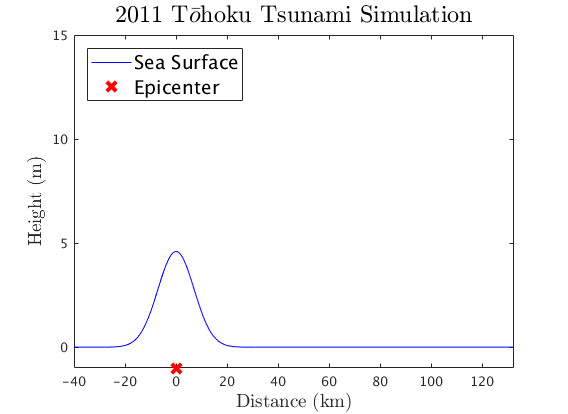
\includegraphics[scale = 0.75]{tsunami_init.png}
\end{figure}

\noindent When the simulation begins, we see the perturbation split into two separate waves, one that travels to the power plant and one that travels away.

\begin{figure}[H]
\centering
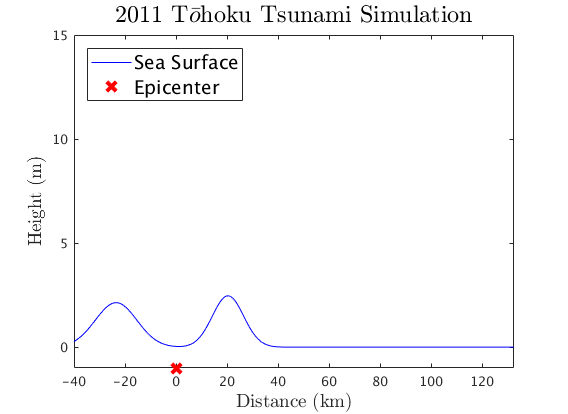
\includegraphics[scale = 0.75]{tsunami_split.png}
\end{figure}


\noindent As the tsunami approaches the power plant, we examine the change in the wave's height.  Reports indicate that the actual tsunami in 2011 reached a height of 15 meters by the time it reached the power plant site \cite{nuclearAssociation}.  In our simulation, we see that when the tsunami's right edge comes in contact with the coast, the tsunami's amplitude reaches 15 meters.

\begin{figure}[H]
\label{tsunamiFinal}
\centering
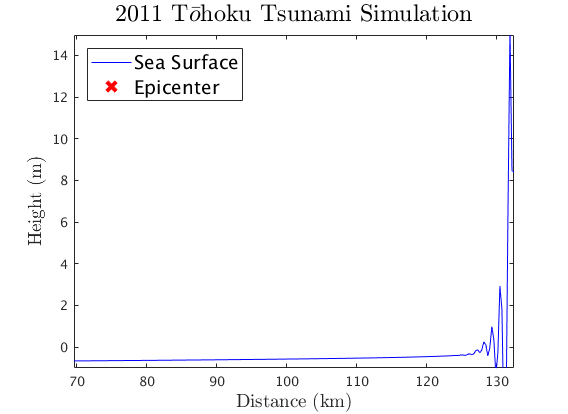
\includegraphics[scale = 0.75]{tsunami_final.png}
\end{figure}

\noindent The simulation also reflects the effects of wave shoaling.  Wave shoaling is an effect that occurs when a wave moves from a deep to shallow region.  Shoaling causes waves to slow, decrease in wavelength, and magnify in amplitude \cite{shoaling}.  This occurs in order to maintain constant energy flux within the wave.  This effect is particularly reflected at the coast, where the seafloor approaches sea level.  In the simulation, we see that the wave's amplitude rapidly increases as it reaches the
coast, which is a direct reflection of wave shoaling.  We also see that shoaling affects the wave traveling away from the power plant as well.  As the seafloor continues to decrease, we see the wave flatten out and increase in speed. \newline


\noindent We also see that in the final frame, there is visible numerical dispersion behind the wavefront.  This is due to our numerical solver, Lax-Wendroff's uses Lax-Friedrich's, which has the Courant-Friedrichs-L\"owy condition:
$$ 1 = \frac{|v|\Delta t}{\Delta x}$$.

\noindent However, in our implementation, the value $|v|$ is computed at the initial time step using current velocity data.  As we have shown previously, velocity changes with time due to shoaling, and the CFL condition is no longer met by our final time step.  This leads to numerical dispersion, as can be seen in \ref{tsunamiFinal}.  In future work, we would like to use an adaptive method so that the CFL condition is always met.  This will control the numerical dispersion and lead to a more accurate model.


\end{document}
